\chapter{Resultados}
\label{chap-results}

Esta Sección presenta un análisis de los resultados obtenidos de la ejecución
del algoritmo sobre distintos videos. A lo largo de esta Sección se refiere al
\textit{algoritmo} como a la versión modificada de contornos activos que fue
descripta en el Capítulo \ref{chap-solution}. Las palabras \textit{aplicación}
y \textit{programa} serán utilizadas indistintamente para referirse al programa
que implementa dicho algoritmo, junto con una interfaz de usuario para el
operador. Se refiere a la\textit{implementación} como a la parte del programa
que implementa el algoritmo.

Se presentan los resultados obtenidos de la ejecución del programa, junto con
métricas utilizadas para evaluar la performance de la implementación.

\section{Aplicación}

El programa incorpora una interfaz gráfica utilizada tanto para dar
instrucciones como para recibir información acerca del partido y del
funcionamiento del algoritmo. La misma cuenta con una sección donde se muestra
una lista de jugadores siendo seguidos, una donde se puede visualizar el video
original con un recuadro en cada jugador seguido, un mapa de calor que muestra
las posiciones más frecuentes, y una imágen que permite al operador evaluar
cualitativamente el correcto funcionamiento del algoritmo.

Para comenzar la ejecución del algoritmo, el programa requiere que el operador
identifique la posición de los jugadores en la imagen inicial de la secuencia.
En este paso, también debe agregar información acerca del número de camiseta
que viste, el equipo, y nombre del jugador.

Un paso adicional que debe ejecutar el operador es determinar los puntos a
utilizar para el cálculo de la homografía. Los datos necesarios para ello son
cuatro parejas de puntos, como explicado en la sección \ref{sec:homography}. De
estas parejas, el primer punto es una coordenada de la imagen en perspectiva y
el otro punto es la coordenada en un plano bidimensional. Con cuatro de estas
relaciones, se puede calcular la matriz que resuelve la homografía para
cualquier otro punto.

Una vez que el programa tiene estos datos, el algoritmo puede comenzar a
su ejecución. Existen dos modos: se puede avanzar un cuadro sólo ante la
indicación del operador (en una mecánica de tipo ``cuadro por cuadro'') y en
otro modo se puede avanzar automáticamente cada vez que se computa un cuadro
(``tiempo real'').

Para cada cuadro, una ventana muestra las posiciones actualizadas de los
jugadores. El usuario puede seleccionar un jugador en particular y ver en
detalle información sobre su posición, velocidad promedio, actual, y máxima
desde el comienzo del seguimiento, y un mapa de calor que muestra con colores
próximos al rojo los lugares más visitados por el jugador. Además, en un
archivo se guarda la posición de cada jugador para cada momento.

De manera opcional, en cada cuadro se guarda en disco duro una copia del estado
actual del seguimiento para referencia futura.

\section{Material utilizado}

Se utilizaron principalmente dos videos, uno correspondiente a un partido entre
los equipos argentinos de los clubes Boca Juniors e Independiente; y un segundo
video en el cual se enfrentan los equipos Independiente y San Lorenzo. Se
detalla a continuación las características de las imágenes extraídas de esos
videos.

\begin{itemize}

  \item \textbf{Boca vs. Independiente:} El video cuenta con una resolución de
    \textit{1080p} (1920 píxeles de ancho y 1080 de alto). La cancha se muestra
    en su totalidad, y se puede observar la totalidad de las gradas del lado
    opuesto y cielo por encima de ellas. Luego de descartar esas regiones del
    video, la resolución pasa a ser de 1459 píxeles de ancho por 304 de alto.
    Se puede apreciar en la Figura \ref{fig:boca-figura} un cuadro del video, luego
    de extracción de las gradas y corrección del efecto de curvatura de la
    lente.

    Los jugadores de Independiente usan remera y shorts de color blanco,
    fácilmente identificables respecto al fondo de color verdoso. El referí, de
    amarillo, también contrasta respecto al fondo. Los jugadores de Boca, por
    otro lado, son difíciles de identificar a la distancia y son confundidos
    con el color del césped de la cancha, como se ilustra en las Figuras
    \ref{fig:boca-dificil-1} y \ref{fig:boca-dificil-2}.

  \item \textbf{Independiente vs. San Lorenzo:} También filmado en resolución de
    \textit{1080p}, las esquinas del campo de juego quedan fuera del campo
    visual. El video recibido ya fue editado y el alto de un cuadro es menor al
    alto de un video en resolución \textit{1080p}. Luego de descartar las
    gradas, la resolución final del video es de 1920 píxeles de ancho y 540 de
    alto. La Figura \ref{fig:independ-figura} muestra un cuadro del video
    procesado.

    Los jugadores de ambos equipos, al utilizar los valores RGB de cada píxel,
    contrastan contra el césped y el algoritmo de contornos activos funciona
    correctamente al analizarlo cualitativamente.

\end{itemize}

\begin{figure}[H]
  \centering
  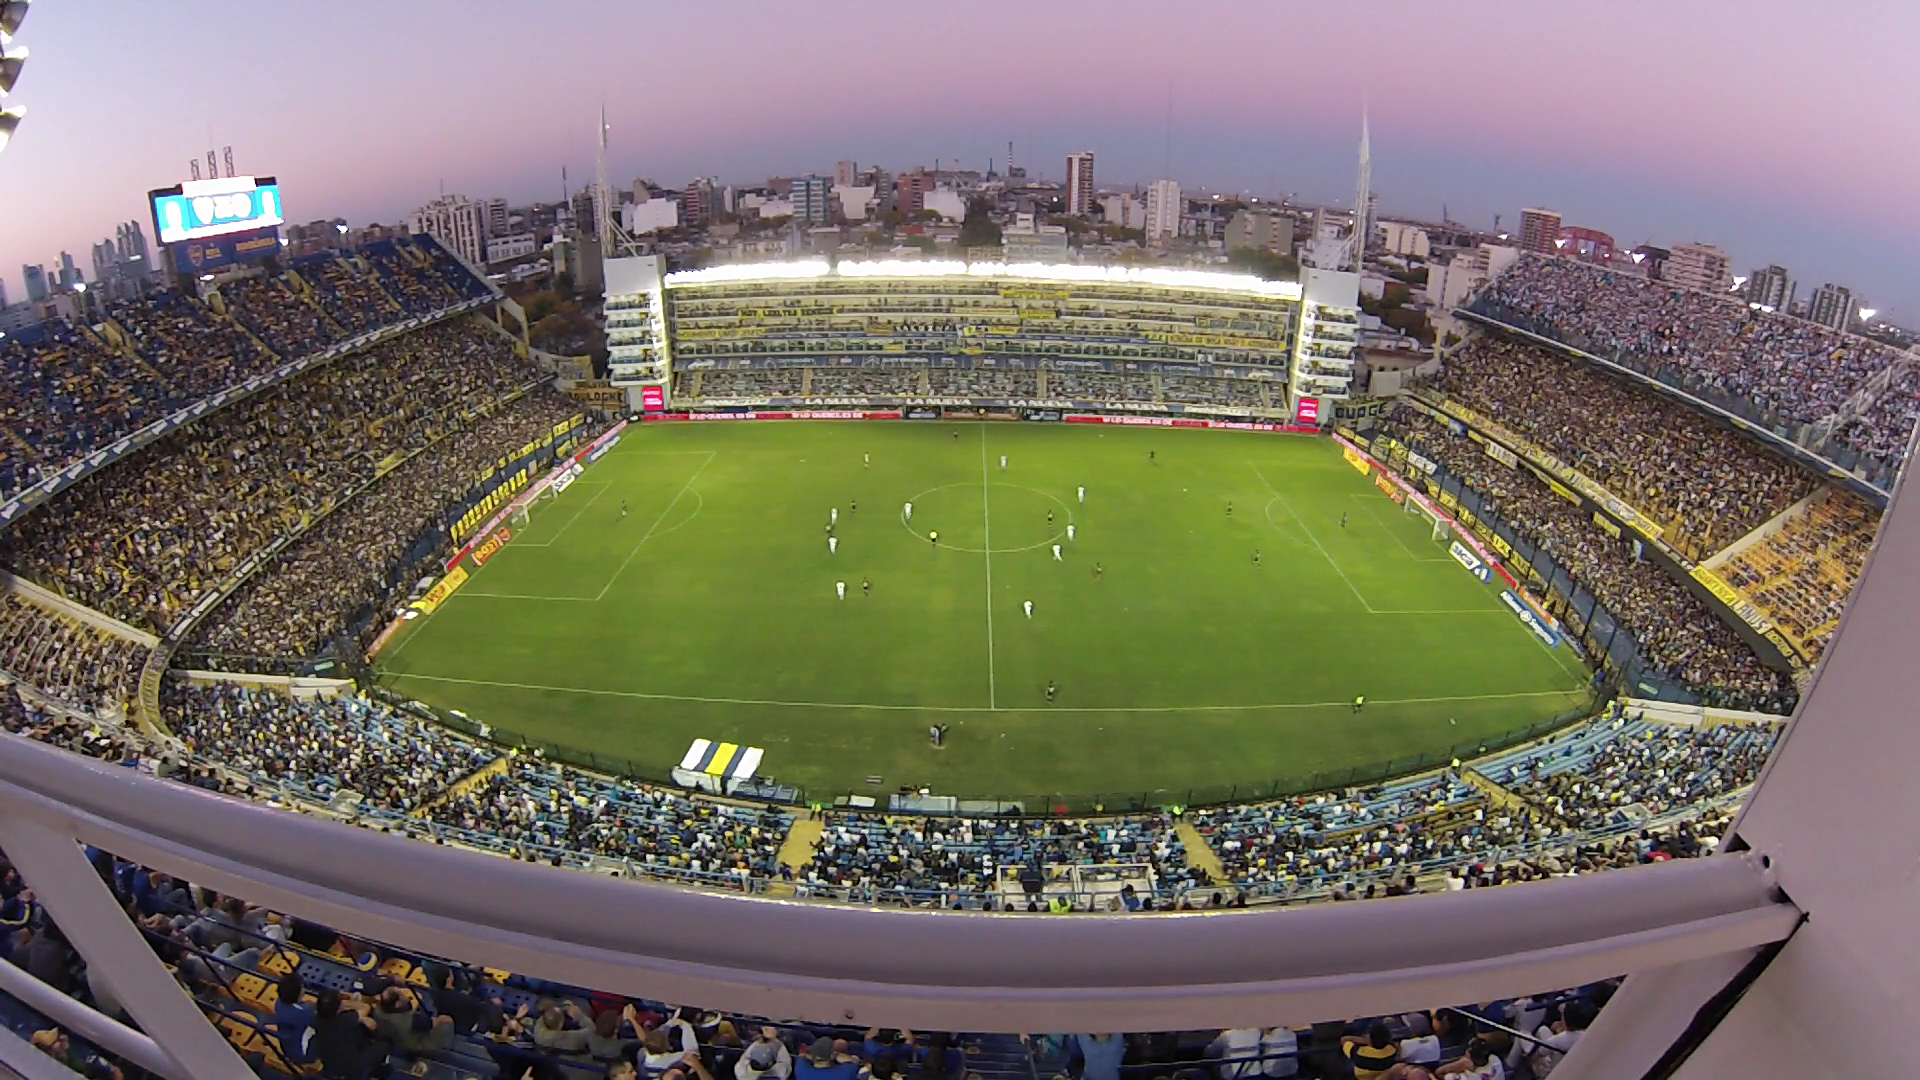
\includegraphics[width=\linewidth]{./images/boca-figura.png}
  \caption{Un cuadro del video de un partido entre Boca e Independiente.}
  \label{fig:boca-figura}
\end{figure}
\begin{figure}[H]
  \centering
  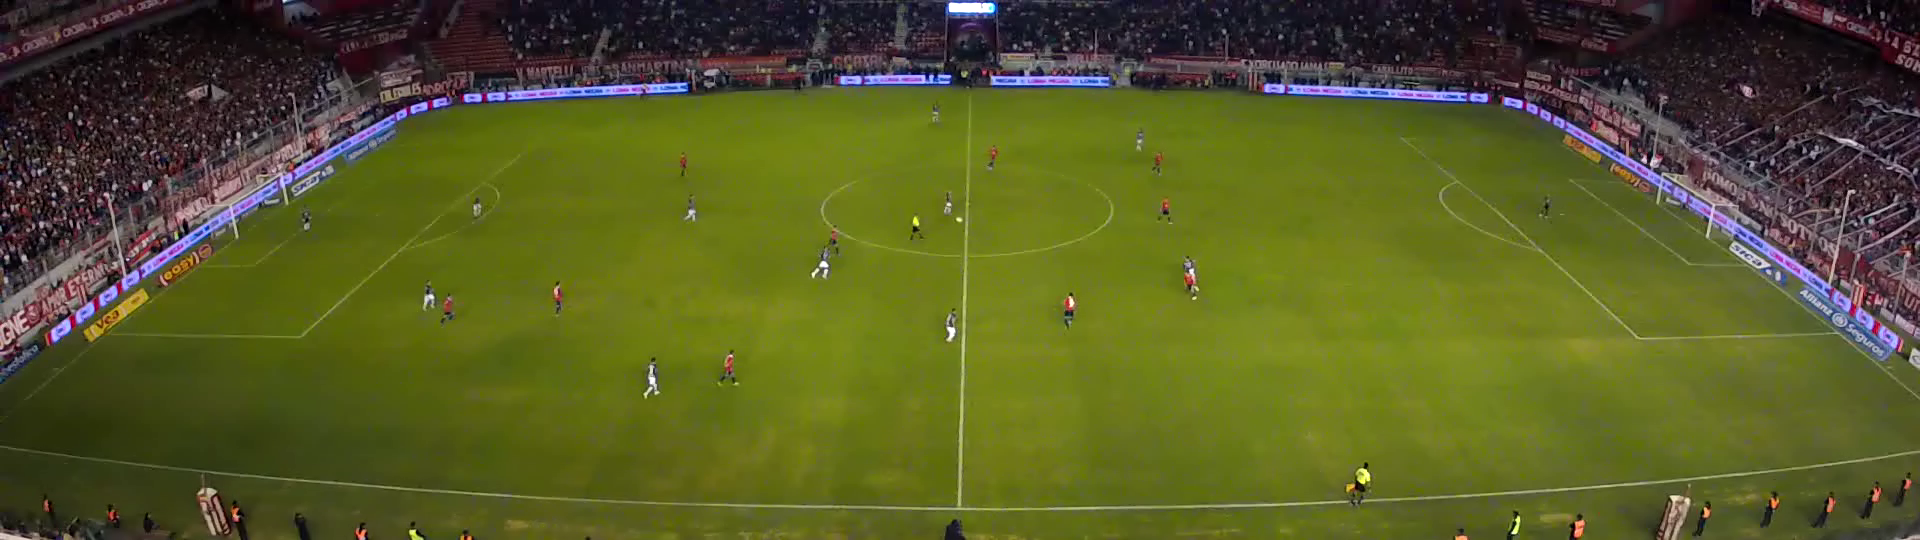
\includegraphics[width=\linewidth]{./images/independ-figura.png}
  \caption{Muestra de un cuadro de un partido en que Independiente enfrenta al club San Lorenzo.}
  \label{fig:independ-figura}
\end{figure}
\begin{figure}[H]
    \centering
    \begin{minipage}[t]{.5\textwidth}
        \centering
        
\includegraphics[width=.4\linewidth]{./images/boca-dificil1.png}
        \label{fig:boca-dificil1}
    \end{minipage}%
    \begin{minipage}[t]{.5\textwidth}
        \centering
        
\includegraphics[width=.4\linewidth]{./images/boca-dificil2.png}
        \label{fig:boca-difícil2}
    \end{minipage}
    \caption{Se muestra un acercamiento a dos jugadores en el video de Boca vs.
             Independiente. Un observador puede notar que los contornos de los
         jugadores son difíciles de delimitar.}

\end{figure}

Además, se tomaron pequeños cortes de tres videos de fútbol televisado en los
cuales la cámara se encuentra relativamente estática y se analizó la
correctitud del seguimiento en estos casos, contando con mayor resolución pero
sin poder efectuar exitosamente la eliminación de fondo o la aplicación de una
homografía para determinar las posiciones correctamente, ya que cada cuadro
donde la cámara cambia su orientación, la matriz de la homografía debería ser
recalculada con nuevos datos.

\begin{itemize}
  \item \textbf{Manchester City vs Barcelona:}

  \item \textbf{Real Madrid vs Borussia Dortmound:}

  \item \textbf{Argentina vs Suiza:}

\end{itemize}

\section{Evaluación del método}

Se evaluó cualitativamente por un operador que los contornos de los jugadores
según el algoritmo modificado de contornos activos no correspondían a los
jugadores, como es el caso de trabajos citados en el estado del arte (ver
\cite{papers-tanos}). Se atribuye esto a la baja calidad de los videos que se
pudieron obtener, y la poca capacidad de procesamiento en comparación.
% TODO: Completar esto justificando mejor -^

Dado esto, se procedió a evaluar cuántas veces sucedía esta discrepancia por
unidad de tiempo. Esta métrica, resumida como la cantidad de errores del
algoritmo por cada cien cuadros, se intentó minimizar durante el estudio de las
variantes de la aplicación.

Otra métrica que se buscó minimizar es el tiempo de demora por cuadro
procesado, hasta intentar alcanzar una velocidad de $24$ cuadros por segundo
(equivalente a $42$ milisegundos por cuadro), la velocidad de los videos
utilizados.

\subsection{Velocidad de Ejecución}

\subsection{Correctitud}

\section{Comparación con IFTrace}
\label{sec:iftrace}

El algoritmo de seguimiento IFTrace, propuesto por \citeauthor*{IFTrace}, es un
algoritmo robusto que soporta cambios de iluminación y forma, oclusiones y se
centra en hallar características representativas de la textura de los objetos a
seguir. Es capaz de recuperarse de errores menores y permite el seguimiento de
múltiples objetos a la vez.

Un algoritmo de este tipo podría proporcionar una solución al problema. Para
comprobarlo, se llevaron a cabo algunas pruebas utilizando un video sintético
creado para este fin, y un video real de un partido de fútbol. En la Figura
\ref{fig:screen1} de la sección anterior se observa un video real. La figura
\ref{fig:sample-happy-occluded} muestra el primer cuadro del video sintético. Pueden
apreciarse a simple vista las marcadas diferencias entre ambos videos, como por
ejemplo la resolución de la imagen y el tamaño y la complejidad de los objetos
de interés.

\begin{figure}[H]
    \centering
    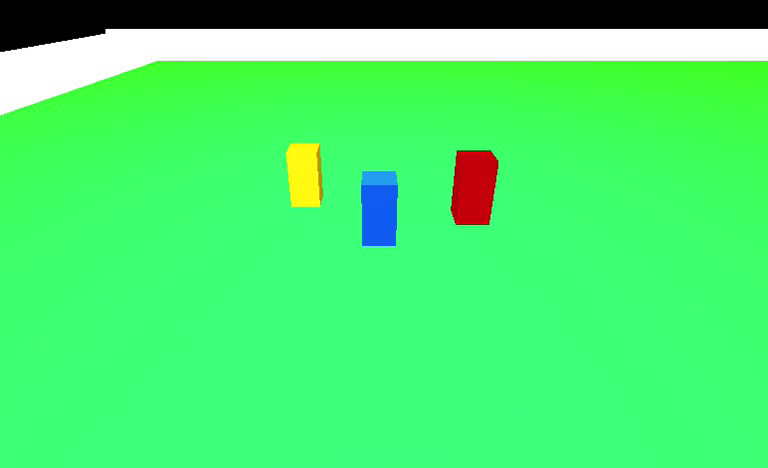
\includegraphics[width=\linewidth]{./images/sample_happy_occluded.png}
    \caption{Muestra de un cuadro del video sintético de prueba.}
    \label{fig:sample-happy-occluded}
\end{figure}

Como se puede ver en la Figura \ref{fig:happy-occluded-iftrace}, IFTrace logra
un correcto seguimiento de múltiples objetos en el video sintético. También
puede observarse, en la Figura \ref{fig:boca-iftrace}, como sigue correctamente
a un jugador en el video real. Sin embargo, el seguimiento sólo es exitoso
durante unos pocos cuadros, ya que, en el cuadro 17, el algoritmo cae en un
error del cual sólo una corrección manual puede sacarlo. Este tipo de corrección
semi-supervisada no está contemplada en el algoritmo de IFTrace.

\begin{figure}[H]
    \centering
    \begin{minipage}[t]{.25\textwidth}
      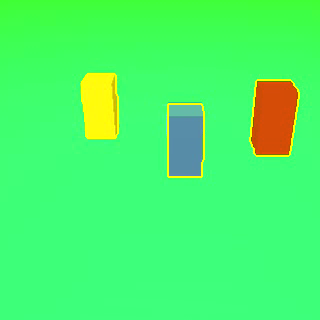
\includegraphics[width=1.4in]{./images/cropped_happy_occluded_00001.png}
      \centering
      \footnotesize
      \textbf{(a)} Cuadro 1
    \end{minipage}
    \hspace{-0.3cm}
    \begin{minipage}[t]{.25\textwidth}
      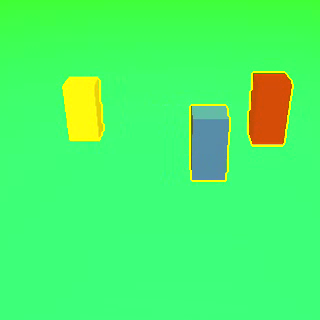
\includegraphics[width=1.4in]{./images/cropped_happy_occluded_00005.png}
      \centering
      \footnotesize
      \textbf{(b)} Cuadro 5
    \end{minipage}
    \hspace{-0.3cm}
    \begin{minipage}[t]{.25\textwidth}
      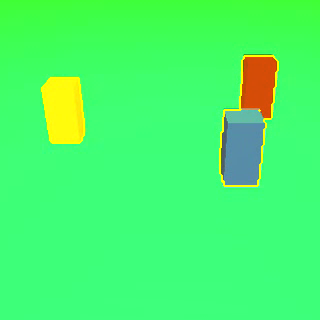
\includegraphics[width=1.4in]{./images/cropped_happy_occluded_00008.png}
      \centering
      \footnotesize
      \textbf{(c)} Cuadro 8
    \end{minipage}
    \hspace{-0.3cm}
    \begin{minipage}[t]{.25\textwidth}
      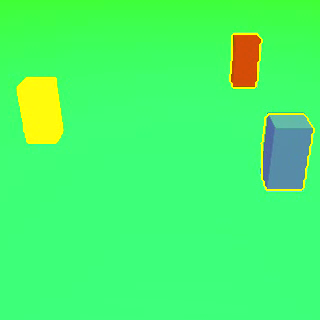
\includegraphics[width=1.4in]{./images/cropped_happy_occluded_00012.png}
      \centering
      \footnotesize
      \textbf{(d)} Cuadro 12
    \end{minipage}
    %% NASTY hack to make refernce work with figures and subfigures, put \label inside \caption env, little bird told me
    \caption{IFTrace funcionando en una secuencia de cuadros de video sintético.
    \label{fig:happy-occluded-iftrace}
    }
\end{figure}

\begin{figure}[H]
    \centering
    \begin{minipage}[t]{.25\textwidth}
      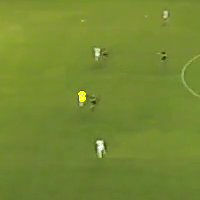
\includegraphics[width=1.4in]{./images/cropped_boca_00009.png}
      \centering
      \footnotesize
      \textbf{(a)} Cuadro 9
    \end{minipage}
    \hspace{-0.3cm}
    \begin{minipage}[t]{.25\textwidth}
      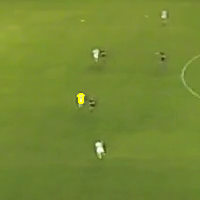
\includegraphics[width=1.4in]{./images/cropped_boca_00012.png}
      \centering
      \footnotesize
      \textbf{(b)} Cuadro 12
    \end{minipage}
    \hspace{-0.3cm}
    \begin{minipage}[t]{.25\textwidth}
      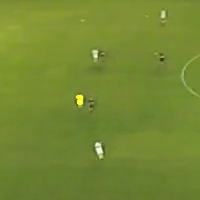
\includegraphics[width=1.4in]{./images/cropped_boca_00014.png}
      \centering
      \footnotesize
      \textbf{(c)} Cuadro 14
    \end{minipage}
    \hspace{-0.3cm}
    \begin{minipage}[t]{.25\textwidth}
      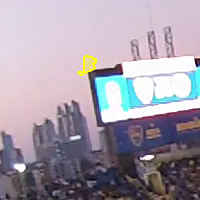
\includegraphics[width=1.4in]{./images/cropped_boca_00017.png}
      \centering
      \footnotesize
      \textbf{(d)} Cuadro 17
    \end{minipage}
    %% NASTY hack to make refernce work with figures and subfigures, put \label inside \caption env, little bird told me
    \caption{Seguimiento de un jugador en un video real utilizando IFTrace.
    \label{fig:boca-iftrace}
    }
\end{figure}

\begin{figure}[H]
    \centering
    \begin{minipage}[t]{.25\textwidth}
      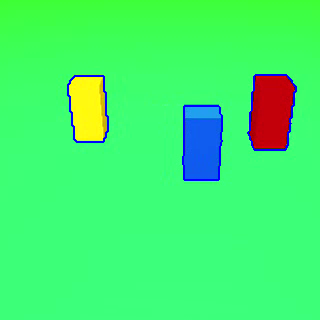
\includegraphics[width=1.4in]{./images/cropped_processing2.png}
      \centering
      \footnotesize
      \textbf{(a)} Cuadro 1
    \end{minipage}
    \hspace{-0.3cm}
    \begin{minipage}[t]{.25\textwidth}
      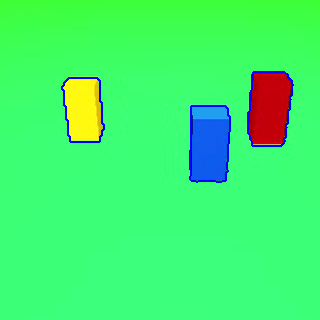
\includegraphics[width=1.4in]{./images/cropped_processing5.png}
      \centering
      \footnotesize
      \textbf{(b)} Cuadro 5
    \end{minipage}
    \hspace{-0.3cm}
    \begin{minipage}[t]{.25\textwidth}
      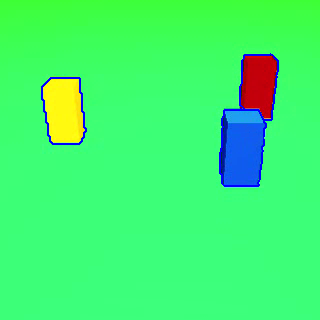
\includegraphics[width=1.4in]{./images/cropped_processing14.png}
      \centering
      \footnotesize
      \textbf{(c)} Cuadro 8
    \end{minipage}
    \hspace{-0.3cm}
    \begin{minipage}[t]{.25\textwidth}
      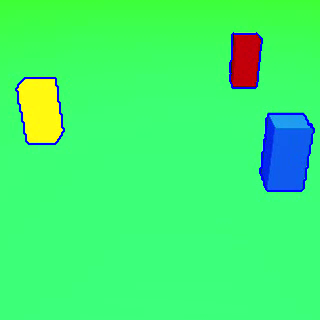
\includegraphics[width=1.4in]{./images/cropped_processing25.png}
      \centering
      \footnotesize
      \textbf{(d)} Cuadro 12
    \end{minipage}
    %% NASTY hack to make refernce work with figures and subfigures, put \label inside \caption env, little bird told me
    \caption{El algoritmo de contornos activos modificado en funcionamiento en un video sintético.
    \label{fig:happy-occluded-activeContour}
    }
\end{figure}

\begin{figure}[H]
    \centering
    \begin{minipage}[t]{.25\textwidth}
      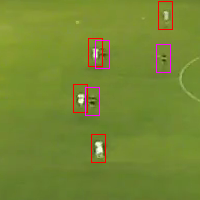
\includegraphics[width=1.4in]{./images/cropped_rendered002.png}
      \centering
      \footnotesize
      \textbf{(a)} Cuadro 2
    \end{minipage}
    \hspace{-0.3cm}
    \begin{minipage}[t]{.25\textwidth}
      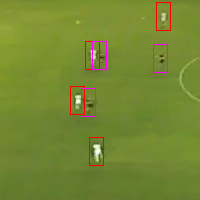
\includegraphics[width=1.4in]{./images/cropped_rendered007.png}
      \centering
      \footnotesize
      \textbf{(b)} Cuadro 12
    \end{minipage}
    \hspace{-0.3cm}
    \begin{minipage}[t]{.25\textwidth}
      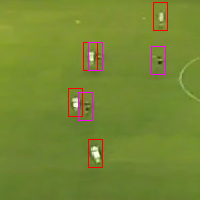
\includegraphics[width=1.4in]{./images/cropped_rendered012.png}
      \centering
      \footnotesize
      \textbf{(c)} Cuadro 14
    \end{minipage}
    \hspace{-0.3cm}
    \begin{minipage}[t]{.25\textwidth}
      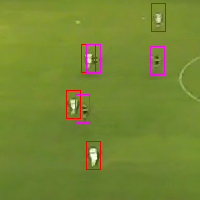
\includegraphics[width=1.4in]{./images/cropped_rendered017.png}
      \centering
      \footnotesize
      \textbf{(d)} Cuadro 17
    \end{minipage}
    %% NASTY hack to make refernce work with figures and subfigures, put \label inside \caption env, little bird told me
    \caption{Seguimiento de los jugadores en un video real mediante el algoritmo de contornos activos modificado.
    \label{fig:boca-activeContour}
    }
\end{figure}

Como se puede observar en la Figura \ref{fig:happy-occluded-activeContour}, el
algoritmo propuesto en este trabajo logra seguir con éxito a los objetos de
interés en el video sintético. Además, también se obtiene un resultado positivo
en el video real en la situación en que IFTrace pierde al jugador, como puede
observarse en la Figura \ref{fig:boca-activeContour}.

\subsection{Evaluación de Comportamiento}

Otro punto importante de comparación entre los dos algoritmos es su tiempo de
ejecución, es decir el tiempo que tarda en llevar a cabo su trabajo.  De
acuerdo a las mediciones realizadas con un video real de un partido de fútbol,
siguiendo a un solo jugador, el tiempo promedio que tarda IFTrace por cuadro es
6.962 segundos, mientras que el algoritmo implementado tiene un tiempo promedio
de 0.712 segundos. Se puede observar que se encuentra un orden magnitud por
debajo de IFTrace, incluso antes de realizar optimizaciones.
%% 6.9628571428571435 si quieren los decimales

Cabe destacar que ambos algoritmos podrían verse beneficiados de ciertas
optimizaciones, como ser por ejemplo la programación en GPU y la reducción de
operaciones de \textit{Input/Output} al almacenamiento secundario (disco duro).

